% #############################################################################
% This is Chapter 6
% !TEX root = ../main.tex
% #############################################################################
% Change the Name of the Chapter i the following line
\fancychapter{Results}
\cleardoublepage
% The following line allows to ref this chapter
\label{chap:conclusion}

This chapter presents the results of our experiments on open-vocabulary aerial image segmentation using the AerialD dataset and RSRefSeg architecture. We analyze both quantitative performance metrics and qualitative segmentation results.

% #############################################################################
\section{Dataset Analysis}

The final AerialD dataset contains a comprehensive collection of aerial images with referring expressions across multiple object categories and spatial relationships.

\begin{figure}[H]
\centering
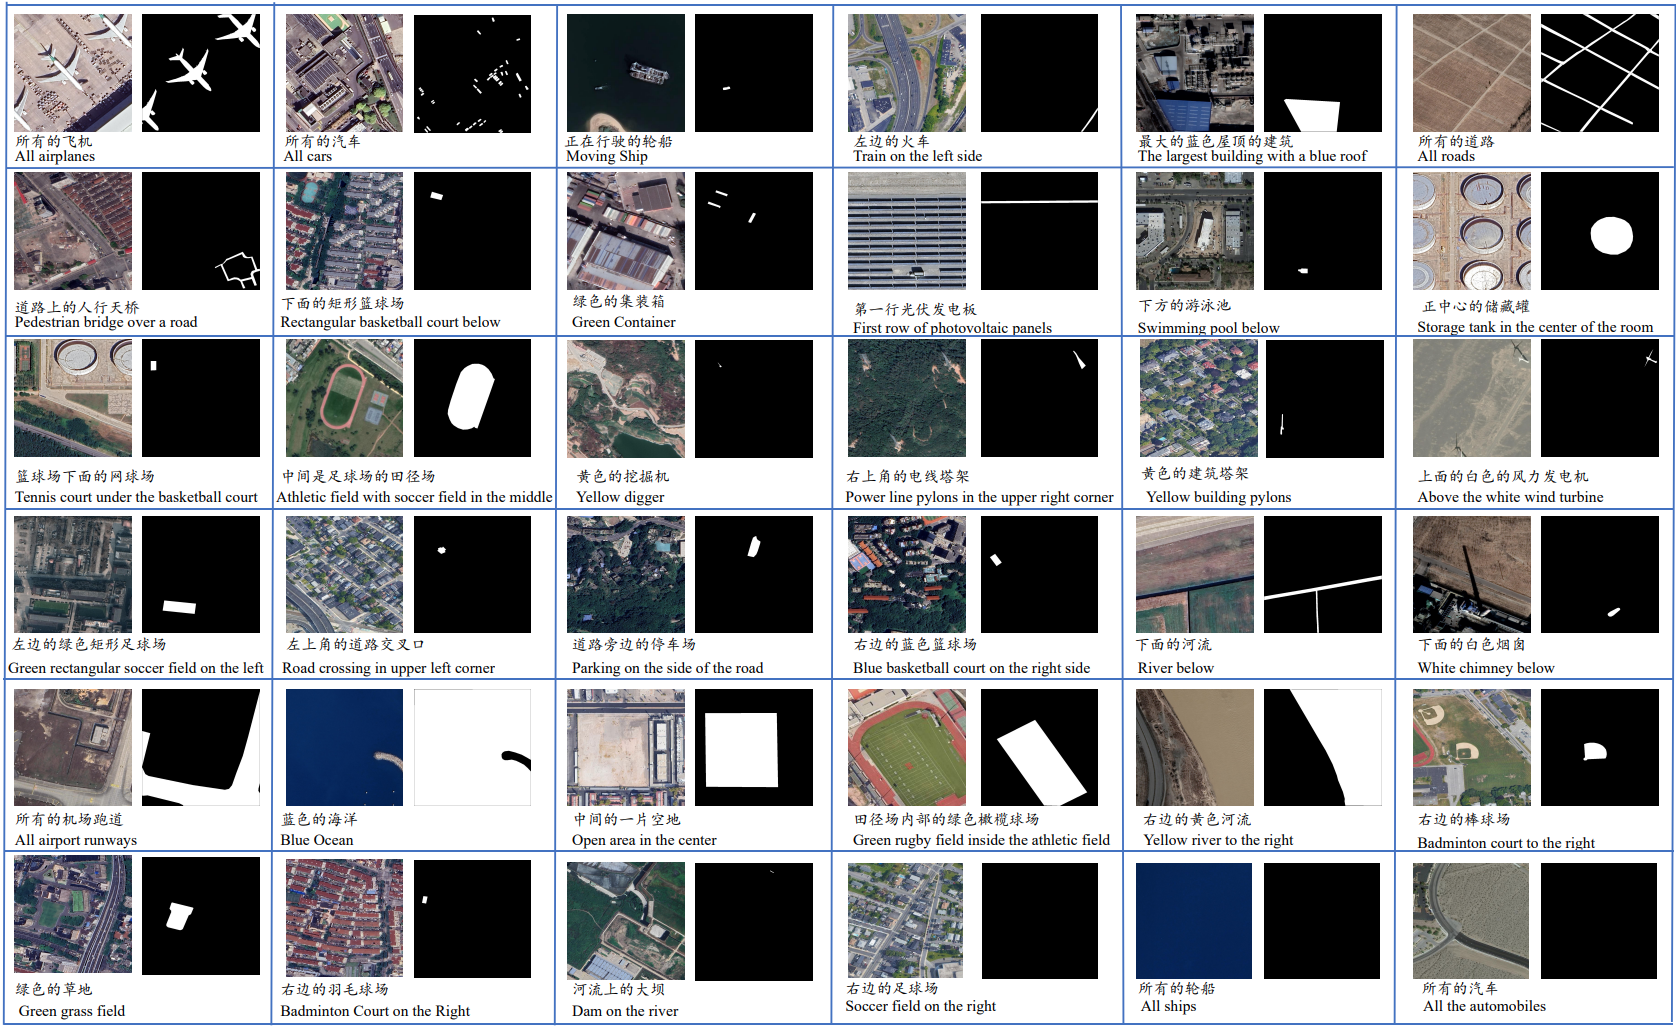
\includegraphics[width=0.8\textwidth]{./Images/dataset.png}
\caption{Dataset Statistics and Composition Analysis}
\label{fig:dataset_stats}
\end{figure}

% #############################################################################
\section{Quantitative Results}
Lorem ipsum dolor sit amet, consectetuer adipiscing elit. Morbi commodo, ipsum sed pharetra gravida, orci magna rhoncus neque, id pulvinar odio lorem non turpis. Nullam sit amet enim. Suspendisse id velit vitae ligula volutpat condimentum. Aliquam erat volutpat. Sed quis velit. Nulla facilisi. Nulla libero. Vivamus pharetra posuere sapien. Nam consectetuer. Sed aliquam, nunc eget euismod ullamcorper, lectus nunc ullamcorper orci, fermentum bibendum enim nibh eget ipsum. Donec porttitor ligula eu dolor. Maecenas vitae nulla consequat libero cursus venenatis. Nam magna enim, accumsan eu, blandit sed, blandit a, eros.

Quisque facilisis erat a dui. Nam malesuada ornare dolor. Cras gravida, diam sit amet rhoncus ornare, erat elit consectetuer erat, id egestas pede nibh eget odio. Proin tincidunt, velit vel porta elementum, magna diam molestie sapien, non aliquet massa pede eu diam. Aliquam iaculis. Fusce et ipsum et nulla tristique facilisis. Donec eget sem sit amet ligula viverra gravida. Etiam vehicula urna vel turpis. Suspendisse sagittis ante a urna. Morbi a est quis orci consequat rutrum. Nullam egestas feugiat felis. Integer adipiscing semper ligula. Nunc molestie, nisl sit amet cursus convallis, sapien lectus pretium metus, vitae pretium enim wisi id lectus. Donec vestibulum. Etiam vel nibh. Nulla facilisi. Mauris pharetra. Donec augue. Fusce ultrices, neque id dignissim ultrices, tellus mauris dictum elit, vel lacinia enim metus eu nunc.

Proin at eros non eros adipiscing mollis. Donec semper turpis sed diam. Sed consequat ligula nec tortor. Integer eget sem. Ut vitae enim eu est vehicula gravida. Morbi ipsum ipsum, porta nec, tempor id, auctor vitae, purus. Pellentesque neque. Nulla luctus erat vitae libero. Integer nec enim. Phasellus aliquam enim et tortor. Quisque aliquet, quam elementum condimentum feugiat, tellus odio consectetuer wisi, vel nonummy sem neque in elit. Curabitur eleifend wisi iaculis ipsum. Pellentesque habitant morbi tristique senectus et netus et malesuada fames ac turpis egestas. In non velit non ligula laoreet ultrices. Praesent ultricies facilisis nisl. Vivamus luctus elit sit amet mi. Phasellus pellentesque, erat eget elementum volutpat, dolor nisl porta neque, vitae sodales ipsum nibh in ligula. Maecenas mattis pulvinar diam. Curabitur sed leo.

Nulla facilisi. In vel sem. Morbi id urna in diam dignissim feugiat. Proin molestie tortor eu velit. Aliquam erat volutpat. Nullam ultrices, diam tempus vulputate egestas, eros pede varius leo, sed imperdiet lectus est ornare odio. Lorem ipsum dolor sit amet, consectetuer adipiscing elit. Proin consectetuer velit in dui. Phasellus wisi purus, interdum vitae, rutrum accumsan, viverra in, velit. Sed enim risus, congue non, tristique in, commodo eu, metus. Aenean tortor mi, imperdiet id, gravida eu, posuere eu, felis. Mauris sollicitudin, turpis in hendrerit sodales, lectus ipsum pellentesque ligula, sit amet scelerisque urna nibh ut arcu. Aliquam in lacus. Vestibulum ante ipsum primis in faucibus orci luctus et ultrices posuere cubilia Curae; Nulla placerat aliquam wisi. Mauris viverra odio. Quisque fermentum pulvinar odio. Proin posuere est vitae ligula. Etiam euismod. Cras a eros.

% #############################################################################
\section{Qualitative Results}

Visual analysis of segmentation results demonstrates the model's capability to accurately identify and segment objects based on natural language descriptions in aerial imagery.

\begin{figure}[H]
\centering
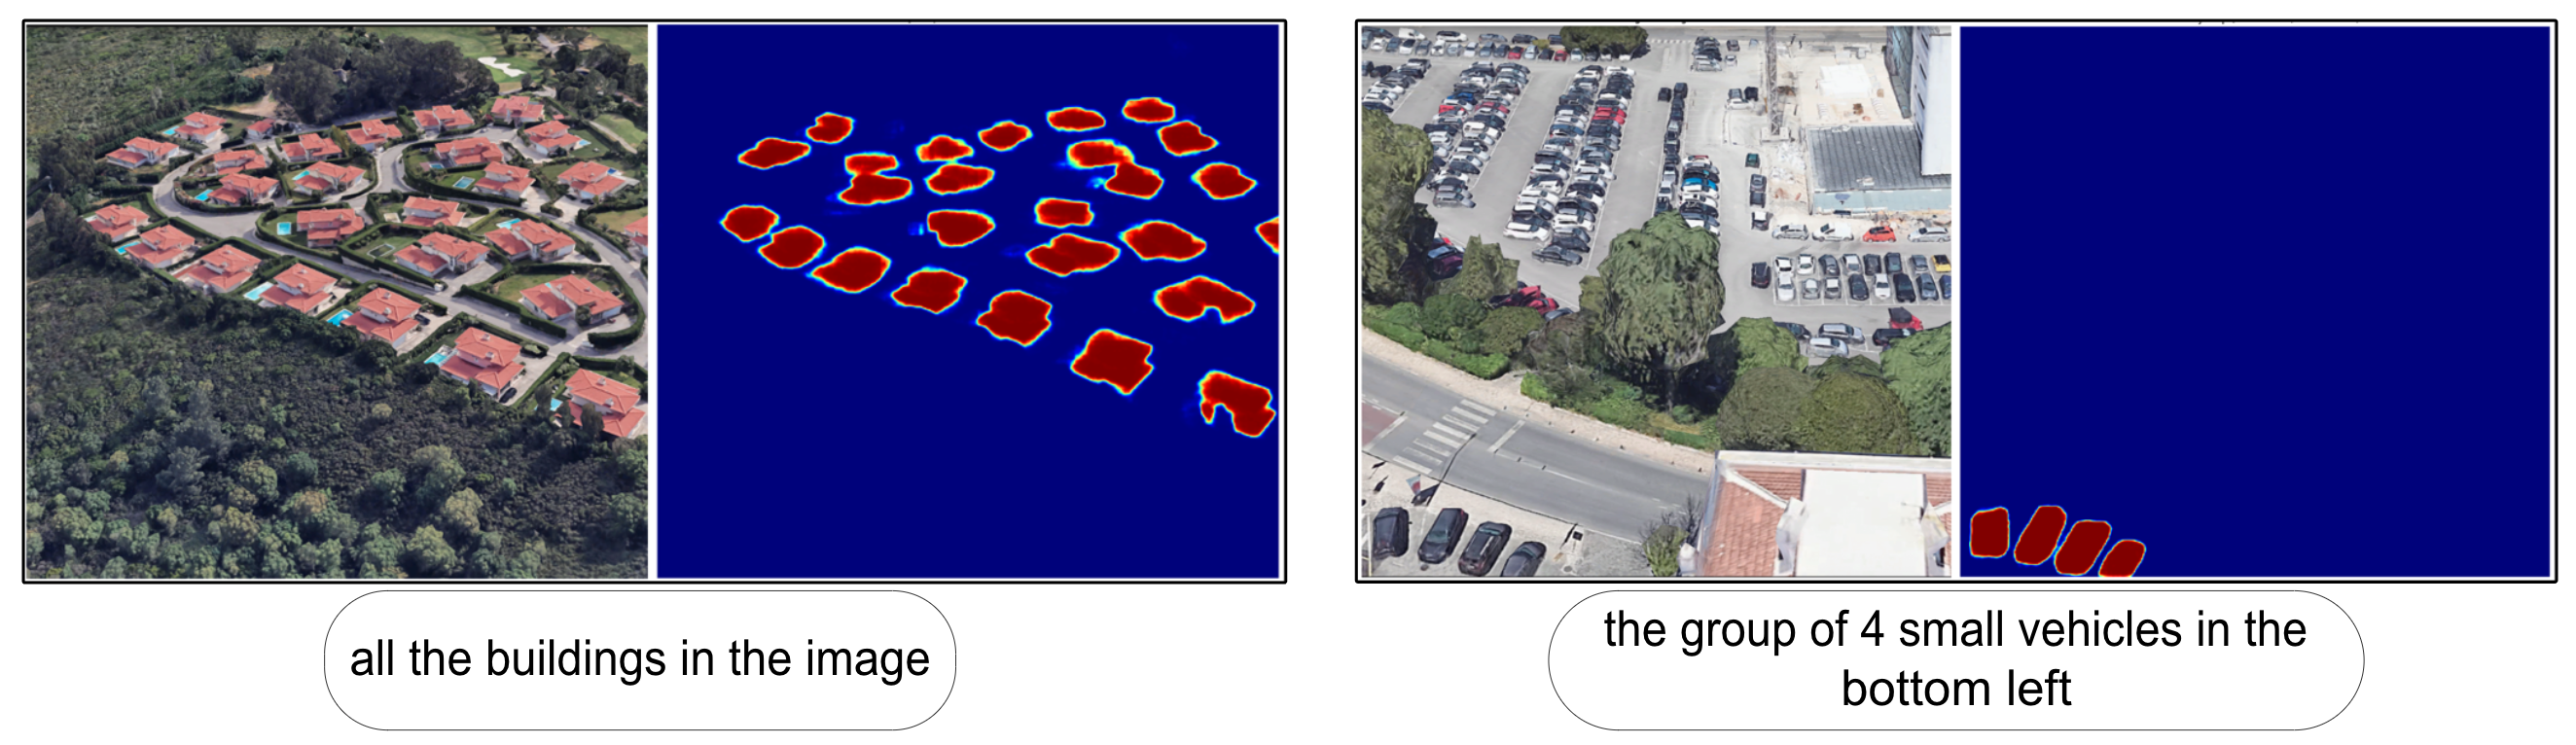
\includegraphics[width=0.9\textwidth]{./Images/qualitative.png}
\caption{Qualitative Segmentation Results on Aerial Images}
\label{fig:qualitative_results}
\end{figure}

The qualitative results show successful segmentation across various object categories including vehicles, buildings, water bodies, and infrastructure elements with varying spatial relationships and contextual descriptions.

% #############################################################################
\section{Analysis and Discussion}
Aliquam aliquet, est a ullamcorper condimentum, tellus nulla fringilla elit, a iaculis nulla turpis sed wisi. Fusce volutpat. Etiam sodales ante id nunc. Proin ornare dignissim lacus. Nunc porttitor nunc a sem. Sed sollicitudin velit eu magna. Aliquam erat volutpat. Vivamus ornare est non wisi. Proin vel quam. Vivamus egestas. Nunc tempor diam vehicula mauris. Nullam sapien eros, facilisis vel, eleifend non, auctor dapibus, pede.